% compile with pdflatex slides.tex

\RequirePackage{atbegshi} 
\documentclass{beamer}
\usepackage[utf8]{inputenc}

% \usepackage{pgfpages}
% \pgfpagesuselayout{4 on 1}[a4paper,landscape,border shrink=5mm]

\usepackage{graphicx}

\usepackage{color}

\usepackage{beamerthemesplit}
\usetheme{progressbar}
\progressbaroptions{headline=sections,frametitle=normal,titlepage=normal}

\usepackage{tikz}
\usetikzlibrary{shapes}
\usetikzlibrary{arrows,decorations.pathmorphing,backgrounds,positioning,fit}
\tikzset{terminal node/.style={circle, draw,
    rounded corners, shade, top color=white, bottom 
    color=blue!50!black!20, draw=blue!40!black!60, thick}}
\tikzset{mdd node/.style={terminal node, rectangle split, rectangle split horizontal, rectangle split parts=#1}}
\tikzset{regular edge/.style={draw=blue!40!black!60, thick}}
\tikzset{outgoing edge/.style={regular edge, very thin}}
\tikzset{comment/.style={blue!95}}
\tikzset{diagram background/.style={fill=blue!2,rounded corners=0.5cm}}

\renewcommand{\O}{\mathrm{O}}
\newcommand{\Z}{\mathbb{Z}}

\title{EVMDD Algorithms for Distance Functions}

\date{August 19, 2010}

\institute{
  \scriptsize
  \vspace{1em}
  École Normale Supérieure de Lyon, France
  (\texttt{pierre.roux@ens-lyon.fr})
  \and
  \vspace{-1em}
  NIA
  (\texttt{radu@nianet.org})
}

\author{
  Pierre~Roux\inst{1}
  \and
  Radu~I.~Siminiceanu\inst{2}
}

%\date{}

\everymath{\displaystyle}

%\includeonlyframes{current}

\begin{document}

\frame{
  \titlepage
}

\frame{\tableofcontents}

%% \AtBeginSection[] 
%% {
%% \begin{frame}<beamer>
%%   \tableofcontents[currentsection]
%% \end{frame}
%% }

\section{BDD}

\begin{frame}
  \frametitle{Model Checking}
  \vspace{-3.2cm}
  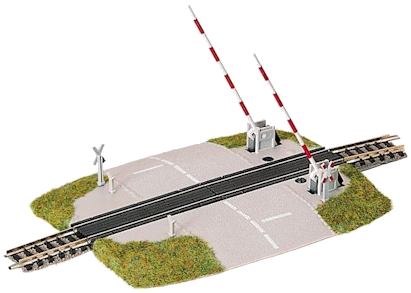
\includegraphics[width=11cm]{railroad_crossing}
  \vspace{-8.2cm}
  \begin{itemize}
  \item States in $\left\{train_l, no\_train_l\right\} \times \left\{barrier\_up, barrier\_down\right\} \times \left\{train_r, no\_train_r\right\}$
  \item Transition relation
    \begin{itemize}
    \item $train_l \rightarrow barrier\_down$
    \item ...
    \end{itemize}
  \end{itemize}
\end{frame}

\begin{frame}
  \frametitle{Representing boolean functions}
  First idea: using trees
  \vspace{-0.5cm}
  \begin{center}
    \hspace{-0.5cm}
    \begin{tikzpicture}
      [xscale=0.75, yscale=1.8, auto]
      \node [mdd node=3]    (l3n0)    at ( 0, 3) {$a$\nodepart{two}0\nodepart{three}1};
      \node [mdd node=3]    (l2n0)    at (-4, 2) {$b$\nodepart{two}0\nodepart{three}1};
      \node [mdd node=3]    (l2n1)    at ( 4, 2) {$b$\nodepart{two}0\nodepart{three}1};
      \node [mdd node=3]    (l1n0)    at (-6, 1) {$c$\nodepart{two}0\nodepart{three}1};
      \node [mdd node=3]    (l1n1)    at (-2, 1) {$c$\nodepart{two}0\nodepart{three}1};
      \node [mdd node=3]    (l1n2)    at ( 2, 1) {$c$\nodepart{two}0\nodepart{three}1};
      \node [mdd node=3]    (l1n3)    at ( 6, 1) {$c$\nodepart{two}0\nodepart{three}1};
      \node [terminal node] (bottom0) at (-7, 0) {0};
      \node [terminal node] (bottom1) at (-5, 0) {1};
      \node [terminal node] (bottom2) at (-3, 0) {0};
      \node [terminal node] (bottom3) at (-1, 0) {1};
      \node [terminal node] (bottom4) at ( 1, 0) {1};
      \node [terminal node] (bottom5) at ( 3, 0) {0};
      \node [terminal node] (bottom6) at ( 5, 0) {0};
      \node [terminal node] (bottom7) at ( 7, 0) {1};
      
      \draw [regular edge]  (l3n0.two   |- l3n0.south) to (l2n0);
      \draw [regular edge]  (l3n0.three |- l3n0.south) to (l2n1);
      \draw [regular edge]  (l2n0.two   |- l2n0.south) to (l1n0);
      \draw [regular edge]  (l2n0.three |- l2n0.south) to (l1n1);
      \draw [regular edge]  (l2n1.two   |- l2n1.south) to (l1n2);
      \draw [regular edge]  (l2n1.three |- l2n1.south) to (l1n3);
      \draw [regular edge]  (l1n0.two   |- l1n0.south) to (bottom0);
      \draw [regular edge]  (l1n0.three |- l1n0.south) to (bottom1);
      \draw [regular edge]  (l1n1.two   |- l1n1.south) to (bottom2);
      \draw [regular edge]  (l1n1.three |- l1n1.south) to (bottom3);
      \draw [regular edge]  (l1n2.two   |- l1n2.south) to (bottom4);
      \draw [regular edge]  (l1n2.three |- l1n2.south) to (bottom5);
      \draw [regular edge]  (l1n3.two   |- l1n3.south) to (bottom6);
      \draw [regular edge]  (l1n3.three |- l1n3.south) to (bottom7);
    \end{tikzpicture}
  \end{center}
  \pause
  \alert{requires $2^n$ terminal nodes}
\end{frame}

\begin{frame}
  \frametitle{Binary Decision Diagram (BDD)}
  \vspace{-0.13cm}
  Merging terminal nodes
  \vspace{-0.5cm}
  \begin{center}
    \hspace{-0.53cm}
    \begin{tikzpicture}
      [xscale=0.75, yscale=1.8, auto]
      \node     [mdd node=3]    (l3n0)    at ( 0, 3) {$a$\nodepart{two}0\nodepart{three}1};
      \node     [mdd node=3]    (l2n0)    at (-4, 2) {$b$\nodepart{two}0\nodepart{three}1};
      \node     [mdd node=3]    (l2n1)    at ( 4, 2) {$b$\nodepart{two}0\nodepart{three}1};
      \node     [mdd node=3]    (l1n0)    at (-6, 1) {$c$\nodepart{two}0\nodepart{three}1};
      \node     [mdd node=3]    (l1n1)    at (-2, 1) {$c$\nodepart{two}0\nodepart{three}1};
      \node     [mdd node=3]    (l1n2)    at ( 2, 1) {$c$\nodepart{two}0\nodepart{three}1};
      \node     [mdd node=3]    (l1n3)    at ( 6, 1) {$c$\nodepart{two}0\nodepart{three}1};
      \node<1>  [terminal node] (bottom0) at (-7, 0) {0};
      \node<1>  [terminal node] (bottom1) at (-5, 0) {1};
      \node<1>  [terminal node] (bottom2) at (-3, 0) {0};
      \node<1>  [terminal node] (bottom3) at (-1, 0) {1};
      \node<1>  [terminal node] (bottom4) at ( 1, 0) {1};
      \node<1>  [terminal node] (bottom5) at ( 3, 0) {0};
      \node<1>  [terminal node] (bottom6) at ( 5, 0) {0};
      \node<1>  [terminal node] (bottom7) at ( 7, 0) {1};
      \node<2-> [terminal node] (bottom0) at (-2, 0) {0};
      \node<2-> [terminal node] (bottom1) at ( 2, 0) {1};

      \draw     [regular edge]  (l3n0.two   |- l3n0.south) to (l2n0);
      \draw     [regular edge]  (l3n0.three |- l3n0.south) to (l2n1);
      \draw     [regular edge]  (l2n0.two   |- l2n0.south) to (l1n0);
      \draw     [regular edge]  (l2n0.three |- l2n0.south) to (l1n1);
      \draw     [regular edge]  (l2n1.two   |- l2n1.south) to (l1n2);
      \draw     [regular edge]  (l2n1.three |- l2n1.south) to (l1n3);
      \draw<1>  [regular edge]  (l1n0.two   |- l1n0.south) to (bottom0);
      \draw<1>  [regular edge]  (l1n0.three |- l1n0.south) to (bottom1);
      \draw<1>  [regular edge]  (l1n1.two   |- l1n1.south) to (bottom2);
      \draw<1>  [regular edge]  (l1n1.three |- l1n1.south) to (bottom3);
      \draw<1>  [regular edge]  (l1n2.two   |- l1n2.south) to (bottom4);
      \draw<1>  [regular edge]  (l1n2.three |- l1n2.south) to (bottom5);
      \draw<1>  [regular edge]  (l1n3.two   |- l1n3.south) to (bottom6);
      \draw<1>  [regular edge]  (l1n3.three |- l1n3.south) to (bottom7);
      \draw<2-> [regular edge]  (l1n0.two   |- l1n0.south) to (bottom0);
      \draw<2-> [regular edge]  (l1n0.three |- l1n0.south) to (bottom1);
      \draw<2-> [regular edge]  (l1n1.two   |- l1n1.south) to (bottom0);
      \draw<2-> [regular edge]  (l1n1.three |- l1n1.south) to (bottom1);
      \draw<2-> [regular edge]  (l1n2.two   |- l1n2.south) to (bottom1);
      \draw<2-> [regular edge]  (l1n2.three |- l1n2.south) to (bottom0);
      \draw<2-> [regular edge]  (l1n3.two   |- l1n3.south) to (bottom0);
      \draw<2-> [regular edge]  (l1n3.three |- l1n3.south) to (bottom1);
    \end{tikzpicture}
  \end{center}
  \visible<3>{still exponential}
  \transdissolve<2>[duration=1]
\end{frame}

\begin{frame}
  \frametitle{BDD cont'd}
  Merging duplicate nodes
  \vspace{-0.5cm}
  \begin{center}
    \hspace{-0.53cm}
    \begin{tikzpicture}
      [xscale=0.75, yscale=1.8, auto]
      \node     [mdd node=3]    (l3n0)    at ( 0, 3) {$a$\nodepart{two}0\nodepart{three}1};
      \node     [mdd node=3]    (l2n0)    at (-4, 2) {$b$\nodepart{two}0\nodepart{three}1};
      \node     [mdd node=3]    (l2n1)    at ( 4, 2) {$b$\nodepart{two}0\nodepart{three}1};
      \node<1>  [mdd node=3]    (l1n0)    at (-6, 1) {$c$\nodepart{two}0\nodepart{three}1};
      \node     [mdd node=3]    (l1n1)    at (-2, 1) {$c$\nodepart{two}0\nodepart{three}1};
      \node     [mdd node=3]    (l1n2)    at ( 2, 1) {$c$\nodepart{two}0\nodepart{three}1};
      \node<1>  [mdd node=3]    (l1n3)    at ( 6, 1) {$c$\nodepart{two}0\nodepart{three}1};
      \node     [terminal node] (bottom0) at (-2, 0) {0};
      \node     [terminal node] (bottom1) at ( 2, 0) {1};

      \draw     [regular edge]  (l3n0.two   |- l3n0.south) to (l2n0);
      \draw     [regular edge]  (l3n0.three |- l3n0.south) to (l2n1);
      \draw<1>  [regular edge]  (l2n0.two   |- l2n0.south) to (l1n0);
      \draw<2-> [regular edge]  (l2n0.two   |- l2n0.south) to (l1n1);
      \draw     [regular edge]  (l2n0.three |- l2n0.south) to (l1n1);
      \draw     [regular edge]  (l2n1.two   |- l2n1.south) to (l1n2);
      \draw<1>  [regular edge]  (l2n1.three |- l2n1.south) to (l1n3);
      \draw<2-> [regular edge]  (l2n1.three |- l2n1.south) to (l1n1);
      \draw<1>  [regular edge]  (l1n0.two   |- l1n0.south) to (bottom0);
      \draw<1>  [regular edge]  (l1n0.three |- l1n0.south) to (bottom1);
      \draw     [regular edge]  (l1n1.two   |- l1n1.south) to (bottom0);
      \draw     [regular edge]  (l1n1.three |- l1n1.south) to (bottom1);
      \draw     [regular edge]  (l1n2.two   |- l1n2.south) to (bottom1);
      \draw     [regular edge]  (l1n2.three |- l1n2.south) to (bottom0);
      \draw<1>  [regular edge]  (l1n3.two   |- l1n3.south) to (bottom0);
      \draw<1>  [regular edge]  (l1n3.three |- l1n3.south) to (bottom1);
    \end{tikzpicture}
  \end{center}
  \visible<3>{exponential in worst case, often better in practice}
  \transdissolve<2>[duration=1]
\end{frame}

\begin{frame}
  \frametitle{BDD end}
  Deleting redundant nodes
  \vspace{-0.5cm}
  \begin{center}
    \hspace{-0.53cm}
    \begin{tikzpicture}
      [xscale=0.75, yscale=1.8, auto]
      \node     [mdd node=3]    (l3n0)    at ( 0, 3) {$a$\nodepart{two}0\nodepart{three}1};
      \visible<1>{
        \node   [mdd node=3]    (l2n0)    at (-4, 2) {$b$\nodepart{two}0\nodepart{three}1};
      }
      \node     [mdd node=3]    (l2n1)    at ( 4, 2) {$b$\nodepart{two}0\nodepart{three}1};
      \node     [mdd node=3]    (l1n1)    at (-2, 1) {$c$\nodepart{two}0\nodepart{three}1};
      \node     [mdd node=3]    (l1n2)    at ( 2, 1) {$c$\nodepart{two}0\nodepart{three}1};
      \node     [terminal node] (bottom0) at (-2, 0) {0};
      \node     [terminal node] (bottom1) at ( 2, 0) {1};

      \draw<1>  [regular edge]  (l3n0.two   |- l3n0.south) to (l2n0);
      \draw<2-> [regular edge]  (l3n0.two   |- l3n0.south) to (l1n1);
      \draw     [regular edge]  (l3n0.three |- l3n0.south) to (l2n1);
      \draw<1>  [regular edge]  (l2n0.two   |- l2n0.south) to (l1n1);
      \draw<1>  [regular edge]  (l2n0.three |- l2n0.south) to (l1n1);
      \draw     [regular edge]  (l2n1.two   |- l2n1.south) to (l1n2);
      \draw     [regular edge]  (l2n1.three |- l2n1.south) to (l1n1);
      \draw     [regular edge]  (l1n1.two   |- l1n1.south) to (bottom0);
      \draw     [regular edge]  (l1n1.three |- l1n1.south) to (bottom1);
      \draw     [regular edge]  (l1n2.two   |- l1n2.south) to (bottom1);
      \draw     [regular edge]  (l1n2.three |- l1n2.south) to (bottom0);
    \end{tikzpicture}
  \end{center}
  \transdissolve<2>[duration=1]
\end{frame}

\begin{frame}
  \frametitle{BDD characteristics}
  \begin{itemize}
  \item canonicity:\\
    two BDD represent the same function iff they are isomorphic
  \item easy computation:\\
    for $f$, $g$ represented by BDDs of size $|f|$ and $|g|$\\
    $f*g$ computed in $\O\left(|f|\,|g|\right)$\\
    using dynamic programming techniques
  \item size of a BDD completely \emph{unrelated} to size
    of represented set
  \end{itemize}
\end{frame}

\section{Building State Space}

\begin{frame}
  \vspace{-0.5em}
  \frametitle{Globally asynchronous,\\locally synchronous models}
  \begin{center}
    \hspace{3.5cm}
    \begin{tikzpicture}
      % table
      \fill [brown]                   (0, 0) circle (2.2cm);
      \foreach \angle/\maincolor/\haircolor in {0/red/yellow, 90/green/black, 180/blue/brown, 270/yellow/brown!60!black} {
        % philosophers
        \fill [rotate=\angle, \maincolor, rounded corners=0.2cm] (3cm, 0cm) ++(-0.25cm, -0.8cm) rectangle ++(0.5cm, 1.6cm);
        \fill [rotate=\angle, \haircolor] (3cm, 0cm) circle (0.4cm);
        % plates
        \fill [rotate=\angle, white] (1.5cm, 0cm) circle (0.6cm);
        \draw [rotate=\angle, black!40] (1.5cm, 0cm) circle (0.4cm);
        % forks
        \fill [rotate=\angle, rotate=45, white!40!black, rounded corners] (1.2cm, 0cm) ++(0cm, -0.15cm) rectangle ++(0.8cm, 0.3cm);
        \fill [rotate=\angle, rotate=45, white!40!black] (1.1cm, 0cm) ++(0cm, -0.2cm) rectangle ++(0.2cm, 0.4cm);
        \foreach \offset in {-0.25cm, -0.05cm, 0.15cm}
        \fill [rotate=\angle, rotate=45, white!40!black, rounded corners=0.05cm] (0.8cm, 0cm) ++(0cm, \offset) rectangle ++(0.5cm, 0.1cm);
      }
    \end{tikzpicture}\\
    \vspace{-6.5cm}
    \hspace{-6cm}
    \begin{minipage}{0.6\linewidth}
      transition relation: disjunction of \emph{events}\\
      $phil_0\_takes\_fork \lor phil_1\_takes\_fork \lor \ldots$\\
      \\
      e.g. \emph{Dining Philosophers}
    \end{minipage}\\
    \vspace{0.6cm}
    \hspace{-6cm}
    \begin{tikzpicture}
      [yscale=1.5]
      \node (ff) at (0, 1) {fork free};
      \node (fu) at (0, 0) {fork used};

      \draw [->] (ff) to [out=235, in=135] (fu);
      \draw [->] (fu) to [out=45, in=315] (ff);
    \end{tikzpicture}\\
    \vspace{0.4cm}
    \hspace{-6cm}
    \begin{tikzpicture}
      [xscale=2, yscale=0.4]
      \node (waiting) at (-1, 0) {waiting};
      \node (fl)      at ( 0, 1) {fork left};
      \node (fr)      at ( 0,-1) {fork right};
      \node [yshift=-0.4cm] (anchor)  at ( 0,-2) {};
      \node (eating)  at ( 1, 0) {eating};

      \draw [->] (waiting) to (fl.west);
      \draw [->] (waiting) to (fr.west);
      \draw [->] (fl.east)      to (eating);
      \draw [->] (fr.east)      to (eating);
      \draw (eating.south)  to [out=270, in=0] (anchor.center);
      \draw [->] (anchor.center)  to [out=180, in=270] (waiting.south);
    \end{tikzpicture}
  \end{center}
\end{frame}

\begin{frame}
  \frametitle{Breadth First Search}

  \begin{tabbing}
    $\;\;$ \= $\;\;$ \= $\;\;$ \= \kill
    \textbf{BFS}($initial\_state$ : BDD, $events$ : BDD list) : BDD\\
    \> $r \gets \emptyset$\\
    \> $frontier \gets initial\_state$\\
    \> \textbf{do}\\
    \> \> $oldr \gets r$\\
    \> \> $next \gets \emptyset$\\
    \> \> \textbf{for all} $e$ \textbf{in} $events$ \textbf{do}\\
    \> \> \> $next \gets next \cup e(frontier)$\\
    \> \> \textbf{done}\\
    \> \> $frontier \gets next \setminus r$\\
    \> \> $r \gets r \cup frontier$\\
    \> \textbf{while} $r \neq oldr$\\
    \> \textbf{return} $r$
  \end{tabbing}
\end{frame}

\begin{frame}
  \frametitle{Alternative BFS}

  \begin{tabbing}
    $\;\;$ \= $\;\;$ \= $\;\;$ \= \kill
    \textbf{BFS}($initial\_state$ : BDD, $events$ : BDD list) : BDD\\
    \> $r \gets initial\_states$\\
    \> \textbf{do}\\
    \> \> $oldr \gets r$\\
    \> \> $next \gets \emptyset$\\
    \> \> \textbf{for all} $e$ \textbf{in} $events$ \textbf{do}\\
    \> \> \> $next \gets next \cup e(r)$\\
    \> \> \textbf{done}\\
    \> \> $r \gets r \cup next$\\
    \> \textbf{while} $r \neq oldr$\\
    \> \textbf{return} $r$
  \end{tabbing}

  Works often \emph{better}\\
  (size of BDD $r$ unrelated to number of encoded states)
\end{frame}

\begin{frame}
  \frametitle{BFS with chaining and saturation}

  \begin{tabbing}
    $\;\;$ \= $\;\;$ \= $\;\;$ \= \kill
    \textbf{BFS}($initial\_state$ : BDD, $events$ : BDD list) : BDD\\
    \> $r \gets \emptyset$\\
    \> \textbf{do}\\
    \> \> $oldr \gets r$\\
    \> \> \textbf{for all} $e$ \textbf{in} $events$ \textbf{do}\\
    \> \> \> $r \gets r \cup e(r)$\\
    \> \> \textbf{done}\\
    \> \textbf{while} $r \neq oldr$\\
    \> \textbf{return} $r$
  \end{tabbing}

  Often a \emph{lot better}\\
  \vspace{1em}
  ultimately:\\
  Saturation: compute \emph{local fixpoints} instead of one global fixpoint
\end{frame}

\begin{frame}
  \frametitle{Saturation vs BFS}

  \vspace{-3.7mm}
  \begin{center}
    \begin{tabular}{|l|r||r||r|r|}
      \hline
      {\footnotesize Model} & \multicolumn{1}{|c||}{\footnotesize Model} & \multicolumn{1}{c||}{\footnotesize Reachable} & {\footnotesize BFS} & {\footnotesize Saturation} \\
      & \multicolumn{1}{|c||}{\footnotesize size}  & \multicolumn{1}{c||}{\footnotesize states}  & {\footnotesize (sec)} & {\footnotesize (sec)} \\
      \hline
      \hline
      {\footnotesize Dining} & 100 & $5\times10^{62}$ &   0.66 &    0.01 \\
      {\footnotesize philosophers} & 1000 & $9\times10^{626}$ & 145.06 &    0.04 \\
      & 10000 & $4\times10^{6269}$ &   --- &   0.43 \\
      \hline
      \hline
      {\footnotesize Round robin} & 50 & $1\times10^{17}$ &    4.63 &    0.12 \\
      {\footnotesize mutual exclusion} & 100 & $3\times10^{32}$ &   104.24 &    1.04 \\
      {\footnotesize protocol} & 200 & $7\times10^{62}$ &   --- &   8.36 \\
      \hline
      \hline
      {\footnotesize Slotted ring} & 20 & $3\times10^{20}$   &  5.79 &    0.03 \\
      {\footnotesize protocol}     & 40 & $4\times10^{41}$  &   258.55 &    0.22 \\
      {\footnotesize}             & 80 & $1\times10^{84}$ &   --- &  1.74 \\
      \hline
    \end{tabular}\\
    On Intel~Core~2, 1.2GHz, 1.5GB mem\\(``---'' means ``out of memory'').
  \end{center}

\end{frame}

\begin{frame}
  \frametitle{Saturation vs BFS}

  \begin{center}
    \begin{tabular}{|l|r||r||r|r|r|}
      \hline
      {\footnotesize Model} & \multicolumn{1}{|c||}{\footnotesize Model} & \multicolumn{1}{c||}{\footnotesize Reachable} & {\footnotesize BFS} & {\footnotesize Saturation} \\
      & \multicolumn{1}{|c||}{\footnotesize size}  & \multicolumn{1}{c||}{\footnotesize states}  & {\footnotesize (sec)} & {\footnotesize (sec)} \\
      \hline
      \hline
      {\footnotesize Kanban} & 40 & $1\times10^{15}$ &   11.11 &    0.06 \\
      {\footnotesize assembly line} & 200 & $3\times10^{22}$ & --- &    8.54 \\
      & 400 & $6\times10^{25}$ &   --- &   90.14 \\
      \hline
      \hline
      {\footnotesize Knights} & 5 & $7\times10^{7}$ & 345.25 &    0.22 \\
      {\footnotesize problem} & 7 & $2\times10^{15}$ &   --- &  2.05 \\
      & 9 & $9\times10^{24}$ &   --- &   9.22 \\
      \hline
      \hline
      {\footnotesize Randomized} & 6 & $2\times10^{6}$ &   4.48 &    0.87 \\
      {\footnotesize leader election} & 8 & $4\times10^{8}$ &   78.76 &  7.48 \\
      {\footnotesize protocol} & 9 & $5\times10^{9}$ &   258.69 &   18.98 \\
      \hline
    \end{tabular}\\
    On Intel~Core~2, 1.2GHz, 1.5GB mem\\(``---'' means ``out of memory'').
  \end{center}
\end{frame}

\section{Distance computation}

\begin{frame}
  \frametitle{Distance function}

  \begin{itemize}
  \item Distance to initial state, useful for:
    \begin{itemize}
    \item knowing the \emph{diameter} of the model (greatest distance)
    \item getting a \emph{shortest counterexample} to a property in temporal logic
    \end{itemize}
    \pause
  \item Implicitly computed by BFS:\\
    at $n$th step, $r = \left\{s \,|\, s \, at \, distance \, at \, most \, n\right\}$
    \pause
  \item But neither by BFS with chaining nor by saturation
  \item A modified version of saturation keeps track of distances\\
    using another data structure: edge valued decision diagrams
  \end{itemize}
\end{frame}

\begin{frame}
  \frametitle{Multiple Terminal BDD (MTBDD)}
  \begin{itemize}
  \item $f : \left\{0, 1\right\}^n \rightarrow \alert<1>{\Z}$
    \pause
  \item Extend BDD to \alert<2>{Multiple Terminal BDD}
    {\normalsize
    \begin{center}
      \begin{figure}
        \begin{tikzpicture}
          [xscale=1, yscale=1.5, auto]
          \node [mdd node=3]    (l3n0)    at ( 0, 2) {$a$\nodepart{two}0\nodepart{three}1};
          \node [mdd node=3]    (l2n0)    at (-2, 1) {$b$\nodepart{two}0\nodepart{three}1};
          \node [mdd node=3]    (l2n1)    at ( 2, 1) {$b$\nodepart{two}0\nodepart{three}1};
          \node [terminal node] (bottom0) at (-3, 0) {0};
          \node [terminal node] (bottom1) at (-1, 0) {1};
          \node [terminal node] (bottom2) at ( 1, 0) {2};
          \node [terminal node] (bottom3) at ( 3, 0) {3};
          
          \draw [regular edge]  (l3n0.two   |- l3n0.south) to (l2n0);
          \draw [regular edge]  (l3n0.three |- l3n0.south) to (l2n1);
          \draw [regular edge]  (l2n0.two   |- l2n0.south) to (bottom0);
          \draw [regular edge]  (l2n0.three |- l2n0.south) to (bottom1);
          \draw [regular edge]  (l2n1.two   |- l2n1.south) to (bottom2);
          \draw [regular edge]  (l2n1.three |- l2n1.south) to (bottom3);
        \end{tikzpicture}
        \caption{$f : (a, b) \mapsto 2a+b$}
      \end{figure}
    \end{center}}
    \pause
  \item Bad if $\mathrm{Img}\left(f\right)$ too big
  \end{itemize}
\end{frame}

\begin{frame}
  \frametitle{Edge Valued DD (EVBDD)}
  \vspace{0.37cm}
  Merging all terminals to 0 and putting values on edges
  \begin{center}
    \hspace{0.52cm}
    \begin{tikzpicture}
      [xscale=1, yscale=1.5, auto]
      \node     [mdd node=3]    (l3n0)     at ( 0, 2) {$a$\nodepart{two}0\nodepart{three}1};
      \node     [mdd node=3]    (l2n0)     at (-2, 1) {$b$\nodepart{two}0\nodepart{three}1};
      \node     [mdd node=3]    (l2n1)     at ( 2, 1) {$b$\nodepart{two}0\nodepart{three}1};
      \node<1>  [terminal node] (bottom0)  at (-3, 0) {0};
      \node<1>  [terminal node] (bottom1)  at (-1, 0) {1};
      \node<1>  [terminal node] (bottom2)  at ( 1, 0) {2};
      \node<1>  [terminal node] (bottom3)  at ( 3, 0) {3};
      \node<2-> [terminal node] (bottomv0) at ( 0, 0) {0};
      
      \draw<1>  [regular edge]  (l3n0.two   |- l3n0.south) to                 (l2n0);
      \draw<1>  [regular edge]  (l3n0.three |- l3n0.south) to                 (l2n1);
      \draw<2-> [regular edge]  (l3n0.two   |- l3n0.south) to node [swap] {0} (l2n0);
      \draw<2-> [regular edge]  (l3n0.three |- l3n0.south) to node        {0} (l2n1);
      \draw<1>  [regular edge]  (l2n0.two   |- l2n0.south) to                 (bottom0);
      \draw<1>  [regular edge]  (l2n0.three |- l2n0.south) to                 (bottom1);
      \draw<1>  [regular edge]  (l2n1.two   |- l2n1.south) to                 (bottom2);
      \draw<1>  [regular edge]  (l2n1.three |- l2n1.south) to                 (bottom3);
      \draw<2-> [regular edge]  (l2n0.two   |- l2n0.south) to node [swap] {0} (bottomv0);
      \draw<2-> [regular edge]  (l2n0.three |- l2n0.south) to node        {1} (bottomv0);
      \draw<2-> [regular edge]  (l2n1.two   |- l2n1.south) to node [swap] {2} (bottomv0);
      \draw<2-> [regular edge]  (l2n1.three |- l2n1.south) to node        {3} (bottomv0);
    \end{tikzpicture}
  \end{center}
  \visible<3->{Result: sum of edge values on path from root to terminal node}\\
  \transdissolve<2>[duration=1]
\end{frame}

\begin{frame}
  \frametitle{EVBDD cont'd}
  \vspace{0.17cm}
  Canonical node: minimum of outgoing edge values is 0
  \begin{center}
    \hspace{0.52cm}
    \begin{tikzpicture}
      [xscale=1, yscale=1.5, auto]
      \node     [mdd node=3]    (l3n0)     at ( 0, 2) {$a$\nodepart{two}0\nodepart{three}1};
      \node     [mdd node=3]    (l2n0)     at (-2, 1) {$b$\nodepart{two}0\nodepart{three}1};
      \node     [mdd node=3]    (l2n1)     at ( 2, 1) {$b$\nodepart{two}0\nodepart{three}1};
      \node     [terminal node] (bottomv0) at ( 0, 0) {0};
      
      \draw     [regular edge]  (l3n0.two   |- l3n0.south) to node [swap] {0} (l2n0);
      \draw<1>  [regular edge]  (l3n0.three |- l3n0.south) to node        {0} (l2n1);
      \draw<2-> [regular edge]  (l3n0.three |- l3n0.south) to node        {2} (l2n1);
      \draw     [regular edge]  (l2n0.two   |- l2n0.south) to node [swap] {0} (bottomv0);
      \draw     [regular edge]  (l2n0.three |- l2n0.south) to node        {1} (bottomv0);
      \draw<1>  [regular edge]  (l2n1.two   |- l2n1.south) to node [swap] {2} (bottomv0);
      \draw<1>  [regular edge]  (l2n1.three |- l2n1.south) to node        {3} (bottomv0);
      \draw<2-> [regular edge]  (l2n1.two   |- l2n1.south) to node [swap] {0} (bottomv0);
      \draw<2-> [regular edge]  (l2n1.three |- l2n1.south) to node        {1} (bottomv0);
    \end{tikzpicture}
  \end{center}
  \transdissolve<2>[duration=1]
\end{frame}

\begin{frame}
  \frametitle{EVBDD end}
  \vspace{0.22cm}
  Merging duplicate nodes
  \begin{center}
    \hspace{0.52cm}
    \begin{tikzpicture}
      [xscale=1, yscale=1.5, auto]
      \node     [mdd node=3]    (l3n0)     at ( 0, 2) {$a$\nodepart{two}0\nodepart{three}1};
      \node     [mdd node=3]    (l2n0)     at (-2, 1) {$b$\nodepart{two}0\nodepart{three}1};
      \visible<1>{
        \node   [mdd node=3]    (l2n1)     at ( 2, 1) {$b$\nodepart{two}0\nodepart{three}1};
      }
      \node     [terminal node] (bottomv0) at ( 0, 0) {0};
      
      \draw     [regular edge]  (l3n0.two   |- l3n0.south) to node [swap] {0} (l2n0);
      \draw<1>  [regular edge]  (l3n0.three |- l3n0.south) to node        {2} (l2n1);
      \draw<2-> [regular edge]  (l3n0.three |- l3n0.south) to node        {2} (l2n0);
      \draw     [regular edge]  (l2n0.two   |- l2n0.south) to node [swap] {0} (bottomv0);
      \draw     [regular edge]  (l2n0.three |- l2n0.south) to node        {1} (bottomv0);
      \draw<1>  [regular edge]  (l2n1.two   |- l2n1.south) to node [swap] {0} (bottomv0);
      \draw<1>  [regular edge]  (l2n1.three |- l2n1.south) to node        {1} (bottomv0);
    \end{tikzpicture}
  \end{center}
  \transdissolve<2>[duration=1]
\end{frame}

\section{Modified algorithms}

\begin{frame}
  \frametitle{Using reachability information}

  \begin{itemize}
  \item Saturation is faster than any distance computation
  \item We can then
    \begin{itemize}
    \item first compute reachable state space
    \item and use it to improve distance computation
    \end{itemize}
  \item simplest idea: don't try to reach a state already known unreachable
  \end{itemize}
\end{frame}

\begin{frame}
  \frametitle{Comparison of algorithms}

  \vspace{-3.7mm}
  \begin{center}
    \begin{tabular}{|l|r||r|r|r|r|}
      \hline
      {\footnotesize Model} & \multicolumn{1}{|c||}{\footnotesize Model} & {\footnotesize BFS} & {\footnotesize Saturation} & {\footnotesize Distance} & {\footnotesize Modified} \\
      & \multicolumn{1}{|c||}{\footnotesize size}  & {\footnotesize (sec)}  & {\footnotesize (sec)}  & {\footnotesize (sec)} & {\footnotesize (sec)} \\
      \hline
      \hline
      {\footnotesize Dining} & 100 & 0.66 & 0.00 & 0.00 & 0.00 \\
      {\footnotesize philosophers} & 1000 & 145.06 & 0.04 & 0.04 & 0.05 \\
      & 10000 & --- & 0.43 & 0.41 & 0.52 \\
      \hline
      \hline
      {\footnotesize Round robin} & 50 & 4.63 & 0.12 & 0.13 & 0.02 \\
      {\footnotesize mutual exclusion} & 100 & 104.24 & 1.04 & 1.08 & 0.08 \\
      {\footnotesize protocol} & 200 & --- &8.36 & 8.30 & 0.37 \\
      \hline
      \hline
      {\footnotesize Slotted ring} & 20 & 5.79 & 0.03 & 0.13 & 0.13 \\
      {\footnotesize protocol}     & 40 & 258.55 & 0.22 & 1.50 & 1.59 \\
      {\footnotesize}             & 80 &   --- &  1.74 & 20.54 & 21.70 \\
      \hline
    \end{tabular}\\
    On Intel~Core~2, 1.2GHz, 1.5GB mem\\(``---'' means ``out of memory'').
  \end{center}

\end{frame}

\begin{frame}
  \frametitle{Comparison of algorithms}

  \vspace{-3.7mm}
  \begin{center}
    \begin{tabular}{|l|r||r|r|r|r|}
      \hline
      {\footnotesize Model} & \multicolumn{1}{|c||}{\footnotesize Model} & {\footnotesize BFS} & {\footnotesize Saturation} & {\footnotesize Distance} & {\footnotesize Modified} \\
      & \multicolumn{1}{|c||}{\footnotesize size}  & {\footnotesize (sec)}  & {\footnotesize (sec)}  & {\footnotesize (sec)} & {\footnotesize (sec)} \\
      \hline
      \hline
      {\footnotesize Kanban} & 40 & 11.11 & 0.06 & 0.08 & 0.10 \\
      {\footnotesize assembly line} & 200 & --- & 8.54 & 10.50 & 10.86 \\
      & 400 & --- & 90.14 & 109.88 & 104.46 \\
      \hline
      \hline
      {\footnotesize Knights} & 5 & 345.25 & 0.22 & --- & --- \\
      {\footnotesize problem} & 7 & --- & 2.05 & --- & --- \\
      & 9 & --- & 9.22 & --- & --- \\
      \hline
      \hline
      {\footnotesize Randomized} & 6 & 4.48 & 0.87 & 2.26 & 2.77 \\
      {\footnotesize leader election}     & 8 & 78.76 & 7.48 & 28.55 & 64.54 \\ 
      {\footnotesize protocol}     & 9 & 258.69 & 18.98 & 168.43 & 284.86 \\
      \hline
    \end{tabular}\\
    On Intel~Core~2, 1.2GHz, 1.5GB mem\\(``---'' means ``out of memory'').
  \end{center}

\end{frame}

\begin{frame}
  \frametitle{Comparison of algorithms}

  \vspace{-3.7mm}
  \begin{center}
    \begin{tabular}{|l|r||r|r|r|r|}
      \hline
      {\footnotesize Model} & \multicolumn{1}{|c||}{\footnotesize Model} & {\footnotesize BFS} & {\footnotesize Saturation} & {\footnotesize Distance} & {\footnotesize Modified} \\
      & \multicolumn{1}{|c||}{\footnotesize size}  & {\footnotesize (sec)}  & {\footnotesize (sec)}  & {\footnotesize (sec)} & {\footnotesize (sec)} \\
      \hline
      \hline
      {\footnotesize Virtual} & 3 & 0.09 & 0.10 & 0.14 & 0.14 \\
      {\footnotesize Filesystem} & 4 & 0.75 & 1.00 & 1.34 & 1.30 \\
      & 5 & 5.04 & 6.35 & 8.29 & 7.84 \\
      \hline
      \hline
      {\footnotesize Runway} & 3, 5, 3 & 0.07 & 0.82 & 1.71 & 0.92 \\
      {\footnotesize Safety} & 4, 6, 4 & 0.17 & 6.53 & 12.63 & 12.68 \\
      {\footnotesize Monitor} & 5, 7, 5 & 0.28 & 26.95 & 66.08 & 53.16 \\
      \hline
      \hline
      {\footnotesize Rubik's} & 2 & 85.78 & 1.92 & --- & --- \\
      {\footnotesize cube} & 3 & --- & ---\footnote{half an hour on another machine with 40GB of RAM} & --- & --- \\
      \hline
    \end{tabular}\\
    On Intel~Core~2, 1.2GHz, 1.5GB mem\\(``---'' means ``out of memory'').
  \end{center}

\end{frame}

\begin{frame}
  \frametitle{Bounded saturation}

  \begin{itemize}
  \item sometimes interested only in ``close'' states
  \item with BFS: stop after $bound$ iterations
  \item with saturation:
    \begin{itemize}
    \item simplest solution: after firing an event,\\
      forget states which are further than $bound$
    \item or: start from initial state at distance $0$ and state space at $bound$\\
      and don't try to fire events which can not make any state closer
    \end{itemize}
  \end{itemize}
\end{frame}

\begin{frame}
  \frametitle{Bounded saturation (poor) results}

  \begin{center}
    \begin{figure}
      \begin{tikzpicture}[scale=2]
        \draw[red] (0, 0) -- (2.2, 2.2);
        \draw plot[only marks,mark=x,mark options={blue}] file {bound_vs_dist.table};
        \draw[->] (0, 0) -- (2.2, 0);
        \draw[->] (0, 0) -- (0, 2.2);
        \node[anchor=south west] at (0, 2.2) {bounded};
        \node[anchor=south east] at (2.2, 0) {unbounded};
      \end{tikzpicture}
      \caption{Bounded vs unbounded saturation}
    \end{figure}
  \end{center}
\end{frame}

\begin{frame}
  \frametitle{Bounded saturation (poor) results, cont'd}

  \begin{center}
    \begin{figure}
      \begin{tikzpicture}[scale=2]
        \draw[red] (0, 0) -- (2.2, 2.2);
        \draw plot[only marks,mark=x,mark options={blue}] file {bound_vs_bfs.table};
        \draw[->] (0, 0) -- (2.2, 0);
        \draw[->] (0, 0) -- (0, 2.2);
        \node[anchor=south west] at (0, 2.2) {bounded};
        \node[anchor=south east] at (2.2, 0) {BFS};
      \end{tikzpicture}
      \caption{Bounded saturation vs BFS}
    \end{figure}
  \end{center}
\end{frame}

\begin{frame}
  \frametitle{Bounded saturation (poor) results, cont'd}

  \begin{center}
    \begin{figure}
      \begin{tikzpicture}[scale=2]
        \draw[red] (0, 0) -- (2.2, 2.2);
        \draw plot[only marks,mark=x,mark options={blue}] file {bound2_vs_dist.table};
        \draw[->] (0, 0) -- (2.2, 0);
        \draw[->] (0, 0) -- (0, 2.2);
        \node[anchor=south west] at (0, 2.2) {bounded};
        \node[anchor=south east] at (2.2, 0) {unbounded};
      \end{tikzpicture}
      \caption{Bounded from state space vs unbounded saturation}
    \end{figure}
  \end{center}
\end{frame}

\begin{frame}
  \frametitle{Bounded saturation (poor) results, end}

  \begin{center}
    \begin{figure}
      \begin{tikzpicture}[scale=2]
        \draw[red] (0, 0) -- (2.2, 2.2);
        \draw plot[only marks,mark=x,mark options={blue}] file {bound2_vs_bfs.table};
        \draw[->] (0, 0) -- (2.2, 0);
        \draw[->] (0, 0) -- (0, 2.2);
        \node[anchor=south west] at (0, 2.2) {bounded};
        \node[anchor=south east] at (2.2, 0) {BFS};
      \end{tikzpicture}
      \caption{Bounded from state space saturation  vs BFS}
    \end{figure}
  \end{center}
\end{frame}

\begin{frame}
  \frametitle{Conclusions}

  \begin{itemize}
  \item considering events affecting same variables as one big event\\
    is often a good idea, but not always
  \item if those events are not merged, order matters
    \pause
  \item saturation with EVBDD is the best to compute distances,\\
    when it works
  \item otherwise, BFS remains the best
    \pause
  \item models on which distance saturation doesn't work\\
    are those with moves in 2D/3D spaces:
    \begin{itemize}
    \item knights on chess board (knights problem)
    \item planes in sky (runway safety monitor)
    \item \ldots
    \end{itemize}
  \item this prevents a good locality of events
  \end{itemize}
\end{frame}

\begin{frame}
  \frametitle{Future directions}

  \begin{itemize}
  \item could reachability information be used to improve BFS ?
  \item 2D/3D efficient encoding
    \begin{itemize}
    \item basic idea: BDD with children in two (or three) directions
    \item appealing but prevents coding of any relation between directions
    \item other ideas to be explored:
      \begin{itemize}
      \item unordered BDDs
      \item hierarchical set decision diagrams
      \end{itemize}
    \end{itemize}
  \end{itemize}
\end{frame}

% * future directions: 2D/3D efficient encoding, bfs speed up with reachability information?

\appendix

\begin{frame}
  \frametitle{Questions}

  \begin{center}
    {\Huge ?}
  \end{center}
\end{frame}

\end{document}
